\chapter{Theoretical Background}\label{chap:theory}
\begin{chapabstract}

    In this chapter, I put physical mechanisms of radio emissions related to our study.
    At low frequencies, we observe free-free (Bremsstrahlung) and synchrotron radiations.
    Both emissions are the continuum emission.
    While the free-free radiation is usually dominant from a galaxy at $30 \sim 200\GHz$, the synchrotron radiation is dominant less than $30\GHz$ (Figure~\ref{fig:Condon1992_figure1}).
\begin{figure}[htbp]
	\centering
	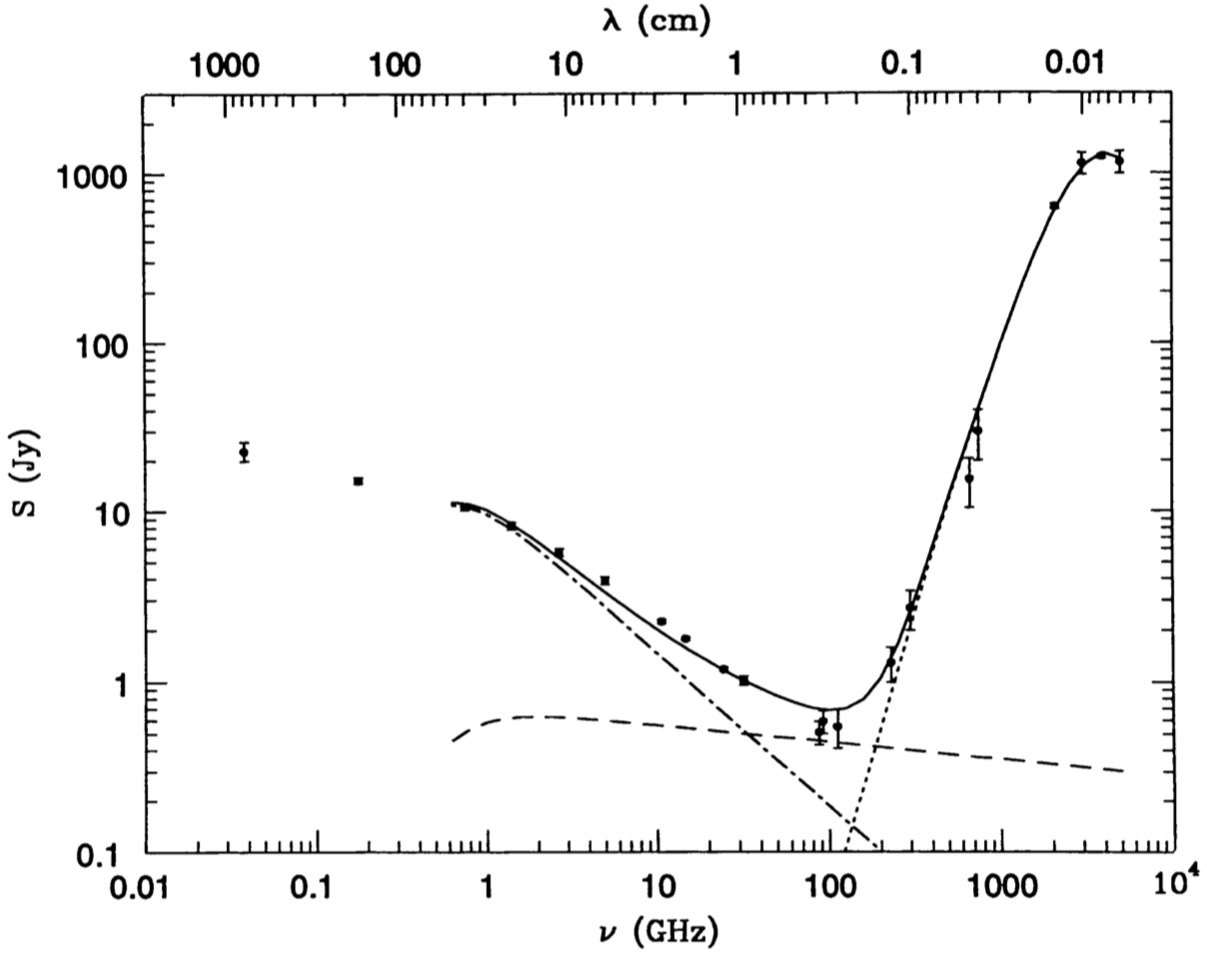
\includegraphics[width=.7\linewidth]{Chapter_2/Figures/Condon1992_Figure1.png}
    \caption[Reprint from \citet{Condon1992a} (Figure~1)]{\label{fig:Condon1992_figure1}
        (Reprint from \citet{Condon1992a}, Figure~1)\\
        This figure shows the spectral energy distribution of M82.
        The dotted line shows the dust thermal emission which is dominant at higher than $200\GHz$.
        The dashed line shows the free-free radiation from the \ih~regions around massive stars,which is dominant at $30 \sim 200\GHz$.
        The dot-dash line shows the synchrotron radiation emitted by the high energy electrons, which is dominant at less than $30\GHz$.
    }
\end{figure}

\end{chapabstract}



\section{Free-free radiation}

The free electrons produce free-free radiation by scattering off ions.
In star-forming galaxies, the radiation source of this emission is the \ih~region where young massive (OB) stars ionized most of the hydrogen atoms.
In this section, we consider the radiation mechanism of free-free radiation.
Here, we consider only electrons emit the radiation because an electron is much more accelerated than an ion due to the difference of their mass (an electron is 1840 times lighter than a proton).

Firstly, I consider the simplest case that a single electron passes by the ion and emits the radiation.
Note that the path of the electron does not change after the interaction because the energy of radio emission is much smaller than the mean electron energy in a plasma.

\begin{equation}\label{eq:essential_radio4n12}
    \frac{E\msb{10\GHz}}{\langle E_e \rangle} = \frac{h \times 10^{10}\,\mr{Hz}}{3kT / 2} = \frac{6.63 \times 10^{-27} \mr{erg\,s} \times 10^{10}\,\mr{Hz}}{1.5 \cdot 1.38 \times 10^{-16}\,\mr{erg\,K^{-1}} \cdot 10^4\,\mr{K}} = 3.3 \times 10^{-5}
\end{equation}

During the interaction, the electron is accelerated by the electric field by the ion.
Then, we can write the equation of motion for parallel and perpendicular to the electron's path (Figure~\ref{fig:nrao_radio4n2}):

\begin{figure}[htbp]
	\centering
	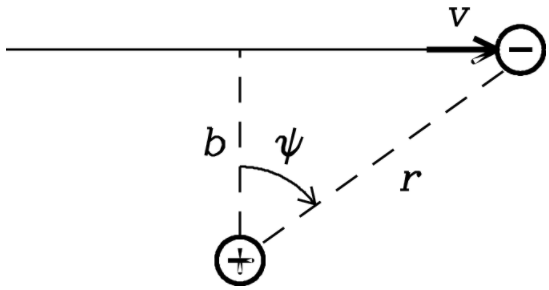
\includegraphics[width=.5\linewidth]{Chapter_2/Figures/NRAO_radio4n2.png}
    \caption[The schematic image of the interaction of an electron with the ion]{\label{fig:nrao_radio4n2}
    }
\end{figure}

\begin{align}
    F_{\|} &= m_{\mr{e}} \dot{v}_{\|}=\frac{-Z e^{2}}{r^{2}} \sin \psi=\frac{-Z e^{2} \sin \psi \cos ^{2} \psi}{b^{2}}\label{eq:essential_radio4n15}\\
    F_{\perp} &= m_{\mr{e}} \dot{v}_{\perp}=\frac{Z e^{2}}{r^{2}} \cos \psi=\frac{Z e^{2} \cos ^{3} \psi}{b^{2}}\label{eq:essential_radio4n16}
\end{align}
where $b$ is the impact parameter and $\cos\psi = \frac{b}{r}$.

These accelerations show different shapes of the pulse (Figure\ref{fig:nrao_radio4n3}).
Since the parallel acceleration produces some infrared radiation with the angular frequency $\omega \sim \tau^{-1} = \frac{v}{b}$ ($tau$ is a collision time), its contribution is negligible at radio frequency.

\begin{figure}[htbp]
	\centering
	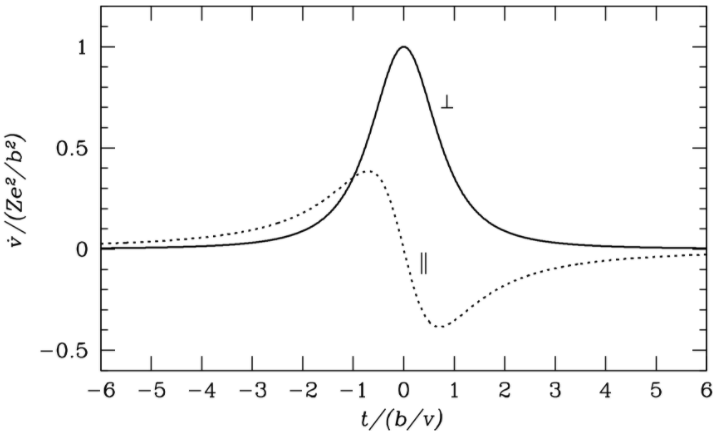
\includegraphics[width=.7\linewidth]{Chapter_2/Figures/NRAO_radio4n3.png}
    \caption[The acceleration of an electron by an ion]{\label{fig:nrao_radio4n3}
    }
\end{figure}

Therefore, the power of free-free radiation from the acceleration of the electron perpendicular to its velocity is:

\begin{equation}\label{eq:essential_radio4n17}
    P=\frac{2}{3} \frac{e^{2} \dot{v}_{\perp}^{2}}{c^{3}}=\frac{2 e^{2}}{3 c^{3}} \frac{Z^{2} e^{4}}{m_{\mr{e}}^{2}}\brp{\frac{\cos ^{3} \psi}{b^{2}}}^{2}
\end{equation}
where we insert $\dot{v}_{\perp}$ into the Larmor's formula $\brp{P = \frac{2}{3}\frac{q^2\dot{v}^2}{c^3},\,q\,\mr{is\,a\,charge}}$, which shows the power emitted by the accelerated particles.

We can get the total energy of $W$ by the pulse as follows:

\begin{equation}\label{eq:essential_radio4n18}
    W = \int^{\infty}_{-\infty} P \mr{d}t
\end{equation}

As I noted above, the electrons' velocity is constant so that we can change of variables:

\begin{equation}\label{eq:essential_radio4n19}
    v = \frac{\rd x}{\rd t}\ \ \ \mr{and}\ \ \ \tan\psi = \frac{x}{b}
\end{equation}

then,

\begin{equation}\label{eq:essential_radio4n20}
    v=\frac{b\,\rd\brp{\tan \psi}}{\rd t}=\frac{b\,\sec ^{2} \psi\,\rd \psi}{\rd t}=\frac{b\,\rd \psi}{\cos ^{2}\psi\,\rd t}
\end{equation}

and

\begin{equation}\label{eq:essential_radio4n21}
    \rd t=\frac{b}{v} \frac{\rd \psi}{\cos ^{2} \psi}
\end{equation}

Substituting Equation~\ref{eq:essential_radio4n17} and~\ref{eq:essential_radio4n21} into Equation~\ref{eq:essential_radio4n18} yields

\begin{equation}\label{eq:essential_radio4n22}
    W=\frac{2}{3} \frac{Z^{2} e^{6}}{c^{3} m_{\mathrm{e}}^{2} b^{4}} \int_{-\pi / 2}^{\pi / 2} \frac{b}{v} \frac{\cos ^{6} \psi}{\cos ^{2} \psi} \rd \psi=\frac{4}{3} \frac{Z^{2} e^{6}}{c^{3} m_{\mathrm{e}}^{2} b^{3} v} \int_{0}^{\pi / 2} \cos ^{4} \psi\ \rd \psi = \frac{\pi Z^2 e^6}{4 c^3 m_{\mr{e}}^2}\brp{\frac{1}{b^3v}}
\end{equation}
where $\int_{0}^{\pi / 2} \cos ^{4} \psi\,\rd \psi=\frac{3 \pi}{16}$.

The pulse energy $W$ shows the total energy emitted by a single electron interaction characterized by the impact parameter $b$ and the electron's velocity $v$.\\ \vspace{0.2cm}

Secondly, I consider the strength and spectral of free-free radiation from \ih~region with several simple assumptions.



\section{Synchrotron radiation}

Synchrotron radiation is a continuum emission which is usually dominant at less than $30\GHz$ in star-forming galaxies.
The interaction of high energy electrons accelerated by the supernova remnant with the galactic magnetic field causes the radiation.
Since high energy electrons have a power-law energy distribution, we call the radiation ``non-thermal synchrotron radiation''.
If electrons have a much smaller velocity than the light, they emit the cyclotron radiation with the cyclotron frequency $\omega = \frac{eB}{m}$ ($e$ is a charge, $B$ is the strength of the magnetic field, $m$ is a mass of an electron).

In this section, I show the mechanism to emit synchrotron radiation.
Firstly, I focus on synchrotron radiation emitted by a single electron.
In the magnetic field with the strength $B$, an electron has a cyclotron frequency $\omega_g = \frac{eB}{m}$
